\documentclass[11pt, a4paper]{article}
\usepackage{float}
\usepackage[utf8]{inputenc}
\usepackage[left=1cm, right=2cm, top=3cm, bottom=3cm, bindingoffset=1cm]{geometry}
\usepackage{csquotes}
\usepackage{subfig}
\usepackage{graphicx}
\usepackage{fancyhdr}
\usepackage{array}
\usepackage[hidelinks]{hyperref}
\usepackage{tcolorbox}
\usepackage{multicol}
\usepackage{amssymb}
\usepackage{enumitem}
\usepackage{longtable}
\usepackage{booktabs}
\usepackage{tabularx}
\usepackage{titlesec}
\usepackage{xcolor}

% Drawings
\usepackage{tikz}
\usetikzlibrary{shapes, arrows, positioning, matrix, calc}

% Metadata
\title{\textbf{Threat Model for ViperVault}}
\author{\textbf{Emanuele Relmi}}
\date{}

% Section formatting
\linespread{1.5}
\pagestyle{fancy}
\fancyhf{}
\fancyhead[C]{\textbf{\nouppercase{\leftmark}}}
\fancyfoot[C]{\thepage}
\renewcommand{\headrulewidth}{1pt}
\renewcommand{\footrulewidth}{1pt}

% Document
\begin{document}
	\maketitle
	\vspace{1cm}
	
	\begin{abstract}
		\noindent This document presents a comprehensive threat model for \textbf{ViperVault}, a password-manager application currently deployed as a native mobile client for Android and iOS.
        The immediate goal of this model is to assess the risks that arise in the current \emph{local-only} configuration of the application, where all data is stored and encrypted directly on the user’s device, with no cloud interaction.
        At the same time, the model anticipates the project’s long-term roadmap, which includes the release of desktop clients (Windows, macOS, Linux), browser extensions and the introduction of a cloud-based synchronization and update service.
        To provide a structured and reproducible analysis, the identified threats are categorized using the \textbf{STRIDE} methodology, ensuring full alignment with industry standards in threat modeling.
        Each threat is described in terms of adversarial action, assessed by likelihood and impact and paired with concrete mitigations that are feasible within the project’s constraints.
        This approach makes it possible to distinguish between immediate device-level risks, such as clipboard hijacking or malware infection and more advanced future threats, such as man-in-the-middle attacks on synchronization, supply-chain compromises or state-sponsored adversaries targeting the backend infrastructure.
        The threat model is further contextualized against major security and privacy frameworks, including \textbf{OWASP}, \textbf{NIST SP~800-63} and European regulatory standards such as \textbf{GDPR} and \textbf{NIS2}.
        By embedding security- and privacy-by-design principles throughout the analysis, ViperVault establishes not only a defensive baseline for the present, but also a forward-looking foundation for sustainable and compliant growth.
        In summary, this document serves both as a snapshot of the current security posture of ViperVault and as a living reference for guiding the project through its future evolution, ensuring that usability, security and regulatory compliance remain in balance at every stage.
	\end{abstract}
	
	\newpage
	\tableofcontents
	\newpage

% Sections
	\section{Scope and Assumptions}
	
	The scope of this threat model is defined around the current and future architecture of \textbf{ViperVault}.
	At present, the application is deployed as a local-only installation on Android and iOS devices.
	All credential data is stored directly on the device and protected through strong cryptographic mechanisms.
	There is no network communication and no persistent cloud storage, which significantly reduces the remote attack surface.
	Looking ahead, however, the project’s roadmap includes several major extensions: the release of desktop clients for Windows, macOS and Linux; the development of browser extensions to facilitate password autofill;  the addition of a cloud synchronization service to enable seamless access across devices.
	These planned features will necessarily expand the system boundaries and introduce new classes of threats that must be considered from the outset.
	In terms of adversaries, the model assumes a broad spectrum of potential threat actors.
	These include opportunistic attackers exploiting common weaknesses, more sophisticated advanced persistent threats (APTs) conducting targeted campaigns, malicious insiders with privileged access and supply-chain adversaries attempting to compromise the build or distribution process.
	The security goals of ViperVault are fourfold.
	First, the confidentiality of all stored credentials must be preserved under every circumstance.
	Second, the integrity of both the vault and its metadata must be ensured, preventing unauthorized tampering.
	Third, the application must remain reliably available to legitimate users.
	Finally, non-repudiation must be enforced for critical operations such as master-password changes, ensuring accountability for sensitive security events.
	The cryptographic foundations of the system rest on well-established and modern primitives.
	The vault is encrypted using the XChaCha20-Poly1305 algorithm, which offers strong authenticated encryption guarantees.
	The master password is processed through Argon2id, a memory-hard key derivation function designed to resist GPU and ASIC cracking attempts.
	All keys are derived exclusively on the user’s device and are never transmitted, in line with zero-knowledge design principles.
	\section{Alignment with Standards and Regulations}
	
	Security and privacy requirements do not exist in isolation: they are guided by community best practices, technical standards and legal frameworks.
	This section places ViperVault in relation to the most relevant reference points, namely the OWASP guidelines, the NIST recommendations and European regulations such as GDPR and NIS2.
	By aligning the threat model with these standards, the project demonstrates not only technical robustness but also regulatory compliance and long-term sustainability.
	
	\subsection{OWASP and NIST}
		
		ViperVault has been designed with explicit reference to the \textbf{OWASP Mobile Application Security Verification Standard (MASVS)} and the \textbf{Mobile Security Testing Guide (MSTG)}.
		Core requirements such as secure credential storage (MASVS-STORAGE-2), strong and up-to-date cryptography, secure input handling and the wiping of sensitive information from memory are explicitly addressed.
		This ensures that the application does not merely rely on cryptographic primitives but also respects best practices for their implementation and for the surrounding environment.
		In addition, the application complies with recommendations from \textbf{NIST SP 800-63B} on digital authentication.
		Specifically, the use of \textbf{Argon2id} as a memory-hard key derivation function satisfies the requirement to resist large-scale GPU or ASIC cracking attempts, while the password policy enforces sufficient entropy, prohibits commonly used secrets and mitigates risks associated with password reuse.
		Together, these controls position ViperVault in line with modern expectations for secure identity and credential management.
	
	\subsection{GDPR}
		
		From a legal and privacy perspective, the design of ViperVault is strongly aligned with the \textbf{General Data Protection Regulation (GDPR)}.
		The application follows the principle of \textbf{Privacy by Design}, meaning that it collects and processes only the minimum data required for its function.
		All vault contents are encrypted client-side, no personal identifiers are stored in plaintext and no unnecessary telemetry or logs are generated.
		The \textbf{right to erasure} is also inherently respected: once a vault is deleted, it is cryptographically unrecoverable, ensuring that the user retains full control over their data lifecycle.
		Furthermore, the principle of \textbf{data minimization} is applied rigorously, with no additional metadata (such as usage statistics or access logs) being collected.
		This not only protects users from privacy risks but also simplifies compliance with regulatory audits.
	
	\subsection{NIS2}
		
		Furthermore, ViperVault is compliant with the European \textbf{NIS2 Directive}, which expands cybersecurity obligations for digital service providers.
		Even though the project is currently developed by a single developer, mechanisms are planned to support a security management lifecycle.
		These include \textbf{reproducible builds} to ensure the integrity of released binaries, a process for responsible \textbf{vulnerability disclosure} and the use of \textbf{digitally signed updates} to prevent tampering.
		In terms of incident response, the project prioritizes transparency and agility.
		Public transparency logs ensure that update integrity can be independently verified and a lightweight process for rapid patching helps minimize exposure when new vulnerabilities are discovered.
		In this way, even with limited resources, ViperVault can embody the spirit of NIS2: resilience, accountability and continuous improvement in security.
	\section{Threat Taxonomy (STRIDE)}
	
	\subsection{Spoofing}
		\begin{center}
			\begin{tabularx}{\textwidth}{>{\raggedright\arraybackslash}p{3cm} | X | c | c | X}
				\toprule
				\textbf{Threat} & \textbf{Description} & \textbf{Likelihood} & \textbf{Impact} & \textbf{Mitigations} \\
				\midrule
				Phishing / Fake App & User tricked into revealing master-password or installing malicious replica. & Medium & High & Code signing, app store integrity, MFA \\
                \midrule
				Biometric Spoofing & Synthetic fingerprint/face sample bypass sensors. & Low & High & Secure enclave validation, liveness detection \\
                \midrule
				WebAuthn Replay & Captured assertion reused. & Low & High & Nonce-based challenges, secure enclave keys \\
				\bottomrule
			\end{tabularx}
		\end{center}
	
	\subsection{Tampering}
		\begin{center}
			\begin{tabularx}{\textwidth}{>{\raggedright\arraybackslash}p{3cm} | X | c | c | X}
				\toprule
				\textbf{Threat} & \textbf{Description} & \textbf{Likelihood} & \textbf{Impact} & \textbf{Mitigations} \\
				\midrule
				Vault File Tampering & Malicious modification of local vault file. & Low & High & Integrity checks, authenticated encryption \\
                \midrule
				DLL / Library Hijacking & Malicious libraries injected. & Low & Medium & Signed libraries, secure load paths \\
                \midrule
				MITM on Sync & Intercept TLS traffic in future sync. & Low (future) & High & TLS 1.3 + certificate pinning \\
                \midrule
				Transparency-Log Forgery & Tampered update manifests. & Low & Critical & Transparency logs, signed manifests \\
				\bottomrule
			\end{tabularx}
		\end{center}
	
	\subsection{Repudiation}
		\begin{center}
			\begin{tabularx}{\textwidth}{>{\raggedright\arraybackslash}p{3cm} | X | c | c | X}
				\toprule
				\textbf{Threat} & \textbf{Description} & \textbf{Likelihood} & \textbf{Impact} & \textbf{Mitigations} \\
				\midrule
				Replay of Reset Tokens & Token reused to regain access. & Low & High & Expiry, signed tokens, vault re-encryption \\
				\bottomrule
			\end{tabularx}
		\end{center}
	
	\subsection{Information Disclosure}
		\begin{center}
			\begin{tabularx}{\textwidth}{>{\raggedright\arraybackslash}p{3cm} | X | c | c | X}
				\toprule
				\textbf{Threat} & \textbf{Description} & \textbf{Likelihood} & \textbf{Impact} & \textbf{Mitigations} \\
				\midrule
				Clipboard Hijacking & Malicious app reads clipboard. & Medium & Medium & Auto-clear clipboard, warnings \\
                \midrule
				Memory Dump / RAM Scraping & Keys extracted from memory. & Low & High & Secure enclave, memory wipe \\
                \midrule
				Unencrypted Backup & Vault stored without encryption. & Medium & High & Force client-side encryption \\
                \midrule
				XSS in Extension & Malicious script steals data. & Low (future) & High & Strict CSP, sandboxed extensions \\
                \midrule
				Side-Channel (Timing, Spectre) & Infer data via timing or speculative execution. & Low & High & Constant-time KDF, patched OS \\
				\bottomrule
			\end{tabularx}
		\end{center}
	
	\subsection{Denial of Service}
		\begin{center}
			\begin{tabularx}{\textwidth}{>{\raggedright\arraybackslash}p{3cm} | X | c | c | X}
				\toprule
				\textbf{Threat} & \textbf{Description} & \textbf{Likelihood} & \textbf{Impact} & \textbf{Mitigations} \\
				\midrule
				Brute Force Lockout & Automated guessing attempts. & Medium & High & KDF cost, rate-limiting \\
                \midrule
				Vault Write Races & Concurrent edits corrupt vault. & Medium & High & File locking, transactional writes \\
                \midrule
				Device Theft or Loss & Loss of unlocked device. & Medium & High & Auto-lock, remote wipe \\
                \midrule
				Overlay / Accessibility DoS & Malicious overlay prevents input. & Low & Medium & Overlay detection, secure flags \\
				\bottomrule
			\end{tabularx}
		\end{center}
	
	\subsection{Elevation of Privilege}
		\begin{center}
			\begin{tabularx}{\textwidth}{>{\raggedright\arraybackslash}p{3cm} | X | c | c | X}
				\toprule
				\textbf{Threat} & \textbf{Description} & \textbf{Likelihood} & \textbf{Impact} & \textbf{Mitigations} \\
				\midrule
				Privilege Escalation & Exploit escape from sandbox. & Low & High & OS hardening, least privilege \\
                \midrule
				Supply-Chain Compromise & Malicious dependency injected. & Low & High & Reproducible builds, signed updates \\
                \midrule
				State-Sponsored APT & Highly resourced adversary. & Low (future) & Critical & Post-quantum crypto, strict E2EE \\
				\bottomrule
			\end{tabularx}
		\end{center}
	\section{Proposed Improvements}
	
	The following enhancements are proposed to strengthen ViperVault’s security posture and to anticipate risks that may emerge as the application evolves. Each improvement is consistent with the principles of security-by-design and privacy-by-design, while remaining feasible for a project developed with limited resources.
	
	\begin{itemize}
		\item \textbf{Duress / Panic Mode}: Introduce an optional mechanism that allows users to configure either a decoy vault or a dedicated “duress password.” This feature is intended for scenarios where a user is coerced into unlocking the application. Under such conditions, entering the duress password would open a harmless decoy vault, thereby protecting the true sensitive data.
		
		\item \textbf{Master Password Reset}: Reinforce the design principle that the master password cannot be trivially reset. In case of loss, the vault should remain inaccessible, which aligns with the zero-knowledge model. To provide a safety net, recovery codes could optionally be generated at first setup and securely stored offline by the user, ensuring that recovery remains possible without weakening overall security.
		
		\item \textbf{Accessibility Overlay Protection}: Implement controls to detect suspicious screen overlays or accessibility abuse. These overlays can be exploited to trick users into interacting with spoofed interfaces. By actively monitoring and blocking untrusted overlays, ViperVault can reduce the risk of visual spoofing and fraudulent input capture.
		
		\item \textbf{Secure Notifications}: Ensure that system notifications never reveal sensitive information. Instead of displaying usernames, vault labels or credential data, notifications should carry only opaque tokens or neutral text, thereby avoiding accidental data leakage through the operating system’s notification channels.
		
		\item \textbf{Anti-Forensics}: Strengthen resistance against forensic attempts by applying multiple safeguards. These include automatic memory wiping when the app is backgrounded, periodic clearing of the clipboard after use and anti-debugging checks that make it harder for adversaries to inspect the application during runtime.
	\end{itemize}
	\section{Future Enhancements: Zero-Knowledge Proofs}
	
	Zero-Knowledge Proofs (ZKP) are not required in the current local-only architecture of ViperVault, since no server-side authentication or interaction exists.
	However, once a synchronization backend and OTA update server are introduced, ZKP-based protocols can provide strong security and privacy advantages.
	
	\subsection{Potential Use Cases}
		\begin{itemize}
			\item \textbf{Server Authentication (Sync/Login)}: Instead of sending password-derived hashes to the server, ViperVault can implement a Password-Authenticated Key Exchange (PAKE) with ZK properties, such as OPAQUE.
			This allows the client to prove knowledge of the master password without revealing it or any verifiable hash to the server.
			\item \textbf{Vault Integrity Proofs}: Clients could prove that uploaded vaults are correctly encrypted under the right key, without disclosing the key itself.
		\end{itemize}
	
	\subsection{Advantages}
		\begin{itemize}
			\item No password hashes or secrets ever stored on the server.
			\item Protection against offline brute-force in case of server breach.
			\item Strong alignment with Zero-Knowledge Architecture principles and GDPR/NIS2 minimization of personal data processing.
			\item Clear FOSS trust signal: the server cannot know secrets even in hashed form.
		\end{itemize}
	
	\subsection{Disadvantages}
		\begin{itemize}
			\item Increased implementation complexity, requiring reliable cryptographic libraries and careful protocol design.
			\item Higher performance cost than traditional logins, especially on low-end devices.
		\end{itemize}
	\section{Diagrams}
	
	\subsection{Current Architecture (Local-Only)}
		\begin{center}
			\resizebox{\textwidth}{!}{
				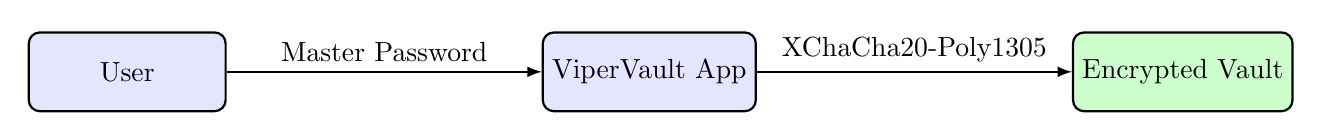
\begin{tikzpicture}[node distance=4cm,>=latex, thick,
					process/.style={rectangle, draw, rounded corners, minimum height=1cm, minimum width=2.5cm, fill=blue!10},
					store/.style={rectangle, draw, rounded corners, minimum height=1cm, minimum width=2.5cm, fill=green!20}, arrow/.style={->, thick}
				]
					
					% Nodes
					\node[process] (user) {User};
					\node[process, right=of user] (app) {ViperVault App};
					\node[store, right=of app] (vault) {Encrypted Vault};
					
					% Arrows
					\draw[arrow] (user) -- (app) node[midway, above]{Master Password};
					\draw[arrow] (app) -- (vault) node[midway, above]{XChaCha20-Poly1305};
				\end{tikzpicture}
			}
		\end{center}
	
	\subsection{Future Architecture (Cloud Sync + Updates)}
		\begin{center}
			\resizebox{\textwidth}{!}{
				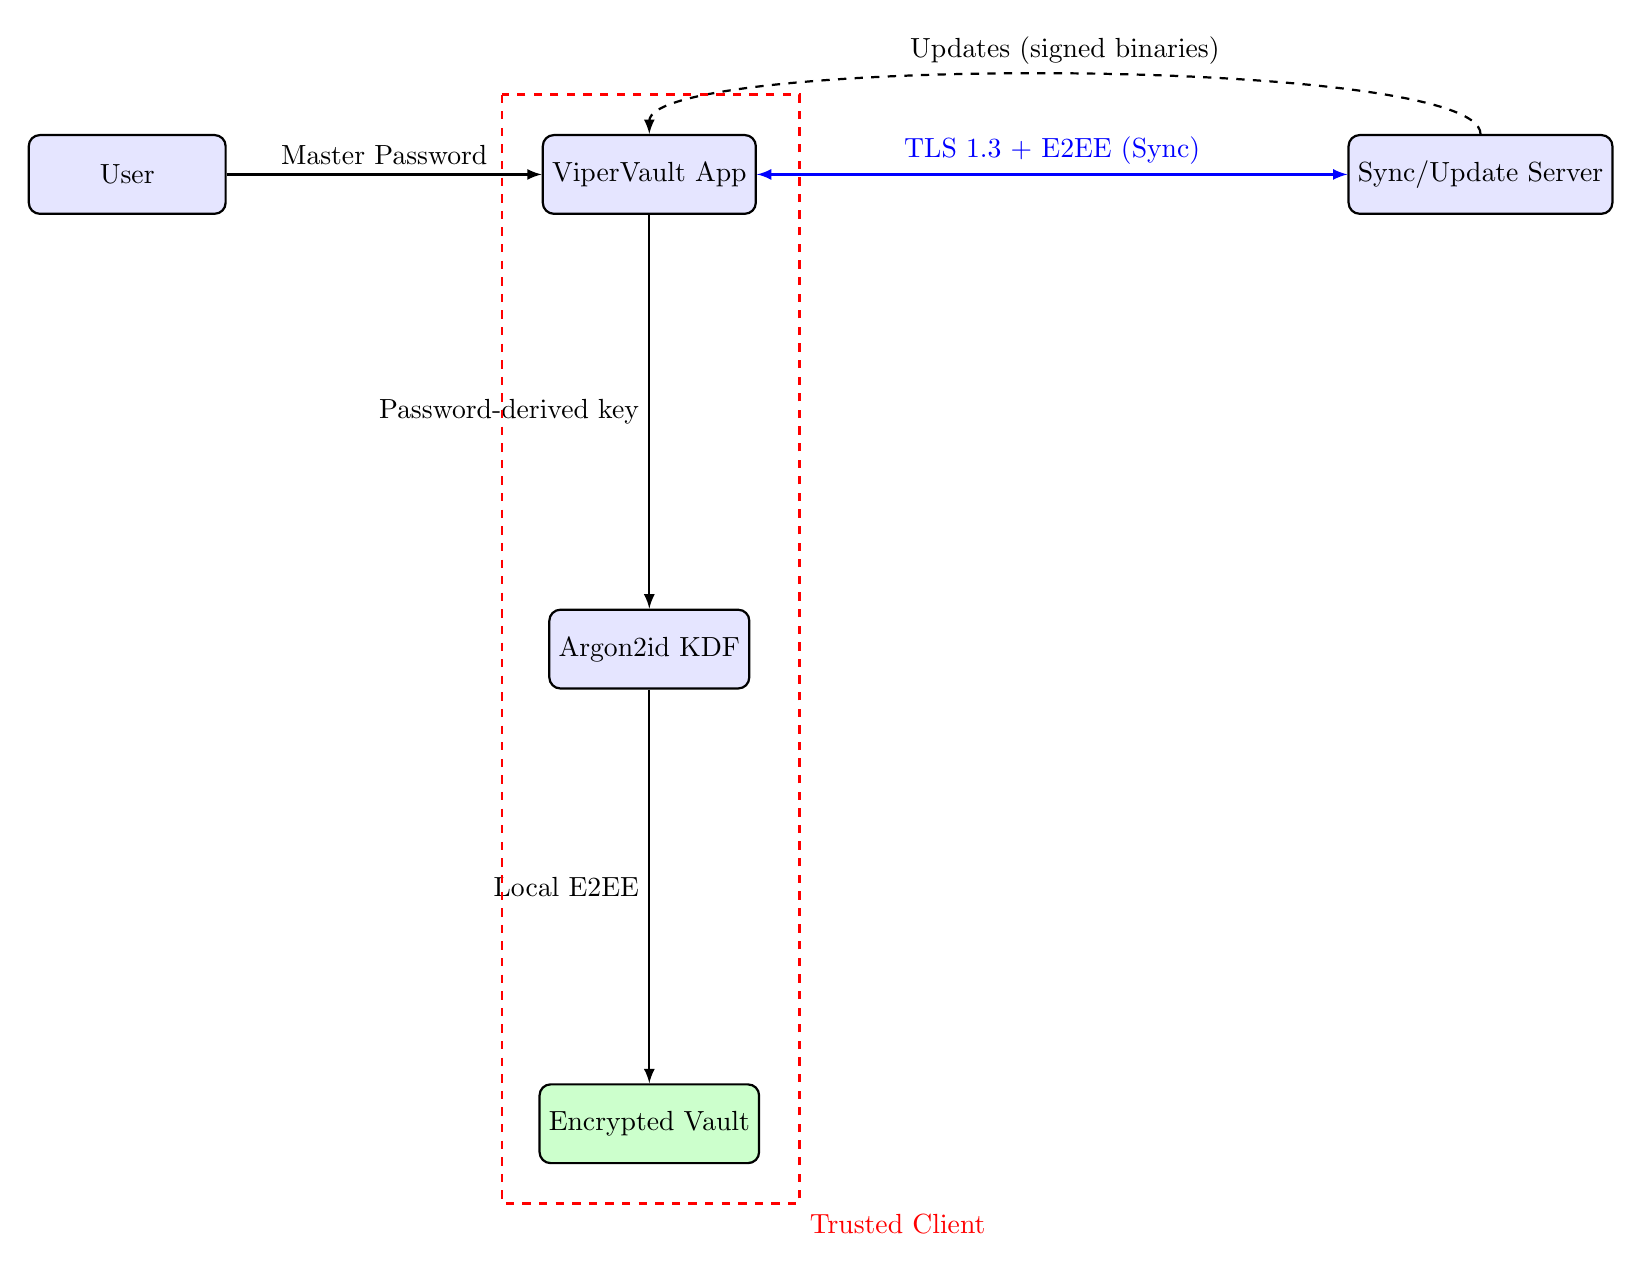
\begin{tikzpicture}
					[node distance=4cm,>=latex, thick,
					process/.style={rectangle, draw, rounded corners, minimum height=1cm, minimum width=2.5cm, fill=blue!10},
					store/.style={rectangle, draw, rounded corners, minimum height=1cm, minimum width=2.5cm, fill=green!20},
					server/.style={rectangle, draw, fill=orange!20, minimum height=1cm, minimum width=2.5cm},
					doublearrow/.style={<->, thick, blue}
					]
					
					% Nodes
					\node[process] (user) {User};
					\node[process, right=of user] (app) {ViperVault App};
					\node[process, below=of app, yshift=-1cm] (kdf) {Argon2id KDF};
					\node[process, right=of app, xshift=3.5cm] (server) {Sync/Update Server};
					\node[store, below=of kdf, yshift=-1cm] (vault) {Encrypted Vault};
					
					% Arrows
					\draw[->] (user) -- (app) node[midway, above]{Master Password};
					\draw[->] (app) -- (kdf) node[midway, left]{Password-derived key};
					\draw[->] (kdf) -- (vault) node[midway, left]{Local E2EE};
					\draw[doublearrow] (app) -- (server) node[midway, above]{TLS 1.3 + E2EE (Sync)};
					\draw[->, dashed] (server.north) .. controls +(up:1cm) and +(up:1cm) .. (app.north) node[midway, above]{Updates (signed binaries)};
					
					% Trust boundary
					\draw[dashed, red] ($(app.north west)+(-0.5,0.5)$) rectangle ($(vault.south east)+(0.5,-0.5)$) node[anchor=north west, red]{Trusted Client};
				\end{tikzpicture}
			}
		\end{center}
	
	\subsection{Encryption Flow}
		\begin{center}
			\resizebox{\textwidth}{!}{
				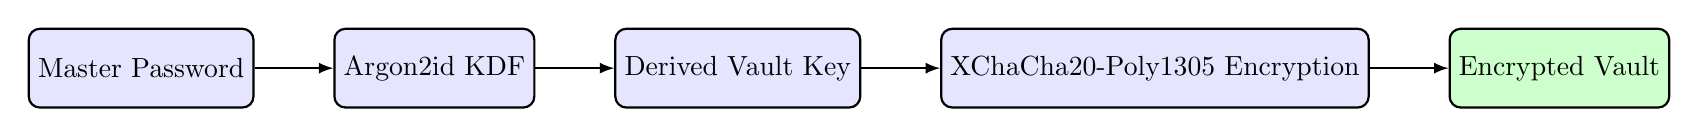
\begin{tikzpicture}[>=latex, thick,
					process/.style={rectangle, draw, rounded corners, minimum height=1cm, minimum width=2.5cm, fill=blue!10},
					store/.style={rectangle, draw, rounded corners, minimum height=1cm, minimum width=2.5cm, fill=green!20},
					arrow/.style={->, thick}
				]
					
					% Nodes
					\node[process] (pw) {Master Password};
					\node[process, right=of pw] (kdf) {Argon2id KDF};
					\node[process, right=of kdf] (key) {Derived Vault Key};
					\node[process, right=of key] (crypto) {XChaCha20-Poly1305 Encryption};
					\node[store, right=of crypto] (vault) {Encrypted Vault};
					
					% Arrows
					\draw[arrow] (pw) -- (kdf);
					\draw[arrow] (kdf) -- (key);
					\draw[arrow] (key) -- (crypto);
					\draw[arrow] (crypto) -- (vault);
				\end{tikzpicture}
			}
		\end{center}
	\section{Conclusion}
	The threat model developed for ViperVault demonstrates a strong alignment with established security and privacy standards, including OWASP, NIST, GDPR and the NIS2 directive.
	At its current stage of development, where the application operates entirely in local-only mode, the most pressing risks are those related to the end-user device itself.
	Examples include the presence of local malware, clipboard hijacking or physical device theft.
	These are threats that can be effectively mitigated with secure enclave usage, automatic vault locking and secure clipboard handling.
	Looking ahead, the planned evolution of ViperVault towards a synchronization server and browser extensions introduces a more complex threat landscape.
	In these future scenarios, the attack surface broadens and more sophisticated adversaries may come into play, such as supply-chain compromises, advanced persistent threats or side-channel attacks.
	Addressing these challenges from the design phase is essential in order to ensure that the transition to a multi-platform, cloud-enabled ecosystem does not erode the strong guarantees already present in the current mobile app.
	The proposed improvements --- such as the introduction of a duress or panic mode, the design of a secure and non-recoverable master password reset mechanism and anti-forensic measures like memory wiping and overlay detection --- further strengthen the defensive posture of the project.
	Combined with ViperVault’s commitment to security- and privacy-by-design principles, these measures provide a clear roadmap for maintaining both user trust and regulatory compliance as the application grows in scope and functionality.
	In conclusion, ViperVault’s threat model not only addresses the risks of the present but also anticipates those of the future, laying down a foundation for a robust, resilient and trustworthy password management solution.

% End
\end{document}